% Options for packages loaded elsewhere
\PassOptionsToPackage{unicode}{hyperref}
\PassOptionsToPackage{hyphens}{url}
%
\documentclass[
  8pt,
  ignorenonframetext,
]{beamer}
\usepackage{pgfpages}
\setbeamertemplate{caption}[numbered]
\setbeamertemplate{caption label separator}{: }
\setbeamercolor{caption name}{fg=normal text.fg}
\beamertemplatenavigationsymbolsempty
% Prevent slide breaks in the middle of a paragraph
\widowpenalties 1 10000
\raggedbottom
\setbeamertemplate{part page}{
  \centering
  \begin{beamercolorbox}[sep=16pt,center]{part title}
    \usebeamerfont{part title}\insertpart\par
  \end{beamercolorbox}
}
\setbeamertemplate{section page}{
  \centering
  \begin{beamercolorbox}[sep=12pt,center]{part title}
    \usebeamerfont{section title}\insertsection\par
  \end{beamercolorbox}
}
\setbeamertemplate{subsection page}{
  \centering
  \begin{beamercolorbox}[sep=8pt,center]{part title}
    \usebeamerfont{subsection title}\insertsubsection\par
  \end{beamercolorbox}
}
\AtBeginPart{
  \frame{\partpage}
}
\AtBeginSection{
  \ifbibliography
  \else
    \frame{\sectionpage}
  \fi
}
\AtBeginSubsection{
  \frame{\subsectionpage}
}
\usepackage{amsmath,amssymb}
\usepackage{lmodern}
\usepackage{iftex}
\ifPDFTeX
  \usepackage[T1]{fontenc}
  \usepackage[utf8]{inputenc}
  \usepackage{textcomp} % provide euro and other symbols
\else % if luatex or xetex
  \usepackage{unicode-math}
  \defaultfontfeatures{Scale=MatchLowercase}
  \defaultfontfeatures[\rmfamily]{Ligatures=TeX,Scale=1}
\fi
% Use upquote if available, for straight quotes in verbatim environments
\IfFileExists{upquote.sty}{\usepackage{upquote}}{}
\IfFileExists{microtype.sty}{% use microtype if available
  \usepackage[]{microtype}
  \UseMicrotypeSet[protrusion]{basicmath} % disable protrusion for tt fonts
}{}
\makeatletter
\@ifundefined{KOMAClassName}{% if non-KOMA class
  \IfFileExists{parskip.sty}{%
    \usepackage{parskip}
  }{% else
    \setlength{\parindent}{0pt}
    \setlength{\parskip}{6pt plus 2pt minus 1pt}}
}{% if KOMA class
  \KOMAoptions{parskip=half}}
\makeatother
\usepackage{xcolor}
\newif\ifbibliography
\usepackage{color}
\usepackage{fancyvrb}
\newcommand{\VerbBar}{|}
\newcommand{\VERB}{\Verb[commandchars=\\\{\}]}
\DefineVerbatimEnvironment{Highlighting}{Verbatim}{commandchars=\\\{\}}
% Add ',fontsize=\small' for more characters per line
\usepackage{framed}
\definecolor{shadecolor}{RGB}{248,248,248}
\newenvironment{Shaded}{\begin{snugshade}}{\end{snugshade}}
\newcommand{\AlertTok}[1]{\textcolor[rgb]{0.94,0.16,0.16}{#1}}
\newcommand{\AnnotationTok}[1]{\textcolor[rgb]{0.56,0.35,0.01}{\textbf{\textit{#1}}}}
\newcommand{\AttributeTok}[1]{\textcolor[rgb]{0.77,0.63,0.00}{#1}}
\newcommand{\BaseNTok}[1]{\textcolor[rgb]{0.00,0.00,0.81}{#1}}
\newcommand{\BuiltInTok}[1]{#1}
\newcommand{\CharTok}[1]{\textcolor[rgb]{0.31,0.60,0.02}{#1}}
\newcommand{\CommentTok}[1]{\textcolor[rgb]{0.56,0.35,0.01}{\textit{#1}}}
\newcommand{\CommentVarTok}[1]{\textcolor[rgb]{0.56,0.35,0.01}{\textbf{\textit{#1}}}}
\newcommand{\ConstantTok}[1]{\textcolor[rgb]{0.00,0.00,0.00}{#1}}
\newcommand{\ControlFlowTok}[1]{\textcolor[rgb]{0.13,0.29,0.53}{\textbf{#1}}}
\newcommand{\DataTypeTok}[1]{\textcolor[rgb]{0.13,0.29,0.53}{#1}}
\newcommand{\DecValTok}[1]{\textcolor[rgb]{0.00,0.00,0.81}{#1}}
\newcommand{\DocumentationTok}[1]{\textcolor[rgb]{0.56,0.35,0.01}{\textbf{\textit{#1}}}}
\newcommand{\ErrorTok}[1]{\textcolor[rgb]{0.64,0.00,0.00}{\textbf{#1}}}
\newcommand{\ExtensionTok}[1]{#1}
\newcommand{\FloatTok}[1]{\textcolor[rgb]{0.00,0.00,0.81}{#1}}
\newcommand{\FunctionTok}[1]{\textcolor[rgb]{0.00,0.00,0.00}{#1}}
\newcommand{\ImportTok}[1]{#1}
\newcommand{\InformationTok}[1]{\textcolor[rgb]{0.56,0.35,0.01}{\textbf{\textit{#1}}}}
\newcommand{\KeywordTok}[1]{\textcolor[rgb]{0.13,0.29,0.53}{\textbf{#1}}}
\newcommand{\NormalTok}[1]{#1}
\newcommand{\OperatorTok}[1]{\textcolor[rgb]{0.81,0.36,0.00}{\textbf{#1}}}
\newcommand{\OtherTok}[1]{\textcolor[rgb]{0.56,0.35,0.01}{#1}}
\newcommand{\PreprocessorTok}[1]{\textcolor[rgb]{0.56,0.35,0.01}{\textit{#1}}}
\newcommand{\RegionMarkerTok}[1]{#1}
\newcommand{\SpecialCharTok}[1]{\textcolor[rgb]{0.00,0.00,0.00}{#1}}
\newcommand{\SpecialStringTok}[1]{\textcolor[rgb]{0.31,0.60,0.02}{#1}}
\newcommand{\StringTok}[1]{\textcolor[rgb]{0.31,0.60,0.02}{#1}}
\newcommand{\VariableTok}[1]{\textcolor[rgb]{0.00,0.00,0.00}{#1}}
\newcommand{\VerbatimStringTok}[1]{\textcolor[rgb]{0.31,0.60,0.02}{#1}}
\newcommand{\WarningTok}[1]{\textcolor[rgb]{0.56,0.35,0.01}{\textbf{\textit{#1}}}}
\setlength{\emergencystretch}{3em} % prevent overfull lines
\providecommand{\tightlist}{%
  \setlength{\itemsep}{0pt}\setlength{\parskip}{0pt}}
\setcounter{secnumdepth}{-\maxdimen} % remove section numbering
\newlength{\cslhangindent}
\setlength{\cslhangindent}{1.5em}
\newlength{\csllabelwidth}
\setlength{\csllabelwidth}{3em}
\newlength{\cslentryspacingunit} % times entry-spacing
\setlength{\cslentryspacingunit}{\parskip}
\newenvironment{CSLReferences}[2] % #1 hanging-ident, #2 entry spacing
 {% don't indent paragraphs
  \setlength{\parindent}{0pt}
  % turn on hanging indent if param 1 is 1
  \ifodd #1
  \let\oldpar\par
  \def\par{\hangindent=\cslhangindent\oldpar}
  \fi
  % set entry spacing
  \setlength{\parskip}{#2\cslentryspacingunit}
 }%
 {}
\usepackage{calc}
\newcommand{\CSLBlock}[1]{#1\hfill\break}
\newcommand{\CSLLeftMargin}[1]{\parbox[t]{\csllabelwidth}{#1}}
\newcommand{\CSLRightInline}[1]{\parbox[t]{\linewidth - \csllabelwidth}{#1}\break}
\newcommand{\CSLIndent}[1]{\hspace{\cslhangindent}#1}
% type setting
% ------------------------------------------------------------------------------
\usepackage[german]{babel}     

% fonts
% ------------------------------------------------------------------------------
\usefonttheme{professionalfonts}

% slide title and horizontal line
% ------------------------------------------------------------------------------
\setbeamertemplate{frametitle}{%
    \vskip-30pt \color{black}\large%
    \begin{minipage}[b][23pt]{120mm}%
    \flushleft\insertframetitle%
    \end{minipage}%
}

\setbeamertemplate{headline}										
{
\vskip10pt\hfill\hspace{3.5mm} 										 
\vskip15pt\color{black}\rule{\textwidth}{0.4pt} 					 
}

% slide number
% ---------------------------------------------------------------
\setbeamertemplate{navigation symbols}{}
\setbeamertemplate{footline}
{
\vskip5pt
\vskip2pt
\makebox[123mm]{\hspace{7.5mm}
\hfill Allgemeines Lineares Modell $\vert$ 
\copyright $ $ 2023 Dirk Ostwald CC BY 4.0 $\vert$ 
Folie \insertframenumber}
\vskip4pt
}

% block color scheme
% ------------------------------------------------------------------------------
% colors
\definecolor{white}{RGB}{255,255,255}
\definecolor{grey}{RGB}{235,235,235}
\definecolor{lightgrey}{RGB}{245,245,245}
\definecolor{LightBlue}{RGB}{220,220,255}
\definecolor{darkblue}{RGB}{51, 51, 153}

% definitions and theorems
\setbeamercolor{block title}{fg = black, bg = grey}
\setbeamercolor{block body}{fg = black, bg = lightgrey}

% general line spacing 
% ------------------------------------------------------------------------------
\linespread{1.3}

% local line spacing
% ------------------------------------------------------------------------------
\usepackage{setspace}

% colors
% -----------------------------------------------------------------------------
\usepackage{color}

% justified text
% ------------------------------------------------------------------------------
\usepackage{ragged2e}
\usepackage{etoolbox}
\apptocmd{\frame}{}{\justifying}{}

% bullet point lists
% -----------------------------------------------------------------------------
\setbeamertemplate{itemize item}[circle]
\setbeamertemplate{itemize subitem}[circle]
\setbeamertemplate{itemize subsubitem}[circle]
\setbeamercolor{itemize item}{fg = black}
\setbeamercolor{itemize subitem}{fg = black}
\setbeamercolor{itemize subsubitem}{fg = black}
\setbeamercolor{enumerate item}{fg = black}
\setbeamercolor{enumerate subitem}{fg = black}
\setbeamercolor{enumerate subsubitem}{fg = black}
\setbeamerfont{itemize/enumerate body}{}
\setbeamerfont{itemize/enumerate subbody}{size = \normalsize}
\setbeamerfont{itemize/enumerate subsubbody}{size = \normalsize}

% color links
% ------------------------------------------------------------------------------
\usepackage{hyperref}
\definecolor{urls}{RGB}{204,0,0}
\hypersetup{colorlinks, citecolor = darkblue, urlcolor = urls}


% additional math commands
% ------------------------------------------------------------------------------
\usepackage{bm}     
\newcommand{\niton}{\not\owns}
\DeclareMathOperator*{\intinf}{\int_{-\infty}^{\infty}}
\DeclareSymbolFont{extraitalic}      {U}{zavm}{m}{it}
\DeclareMathSymbol{\Qoppa}{\mathord}{extraitalic}{161}
\DeclareMathSymbol{\qoppa}{\mathord}{extraitalic}{162}

% text highlighting
% ------------------------------------------------------------------------------
\usepackage{soul}
\makeatletter
\let\HL\hl
\renewcommand\hl{%
  \let\set@color\beamerorig@set@color
  \let\reset@color\beamerorig@reset@color
  \HL}
\makeatother

% equation highlighting
% -----------------------------------------------------------------------------
\newcommand{\highlight}[2][yellow]{\mathchoice%
  {\colorbox{#1}{$\displaystyle#2$}}%
  {\colorbox{#1}{$\textstyle#2$}}%
  {\colorbox{#1}{$\scriptstyle#2$}}%
  {\colorbox{#1}{$\scriptscriptstyle#2$}}}%

% additional mathematical operators
% ------------------------------------------------------------------------------
\DeclareMathOperator*{\argmax}{arg\,max}
\DeclareMathOperator*{\argmin}{arg\,min}

\ifLuaTeX
  \usepackage{selnolig}  % disable illegal ligatures
\fi
\IfFileExists{bookmark.sty}{\usepackage{bookmark}}{\usepackage{hyperref}}
\IfFileExists{xurl.sty}{\usepackage{xurl}}{} % add URL line breaks if available
\urlstyle{same} % disable monospaced font for URLs
\hypersetup{
  hidelinks,
  pdfcreator={LaTeX via pandoc}}

\author{}
\date{\vspace{-2.5em}}

\begin{document}

\begin{frame}[plain]{}
\protect\hypertarget{section}{}
\center

\begin{center}
\includegraphics[width=0.2\linewidth]{7_Abbildungen/alm_7_otto} \end{center}

\vspace{2mm}

\huge

Allgemeines Lineares Modell \vspace{6mm}

\large

BSc Psychologie SoSe 2023

\vspace{6mm}
\normalsize

Prof.~Dr.~Dirk Ostwald
\end{frame}

\begin{frame}[plain]{}
\protect\hypertarget{section-1}{}
\center
\huge
\vfill

\noindent (7) T-Statistiken \vfill
\end{frame}

\begin{frame}{}
\protect\hypertarget{section-2}{}
\large

Naturwissenschaft \vspace{7mm}

\begin{center}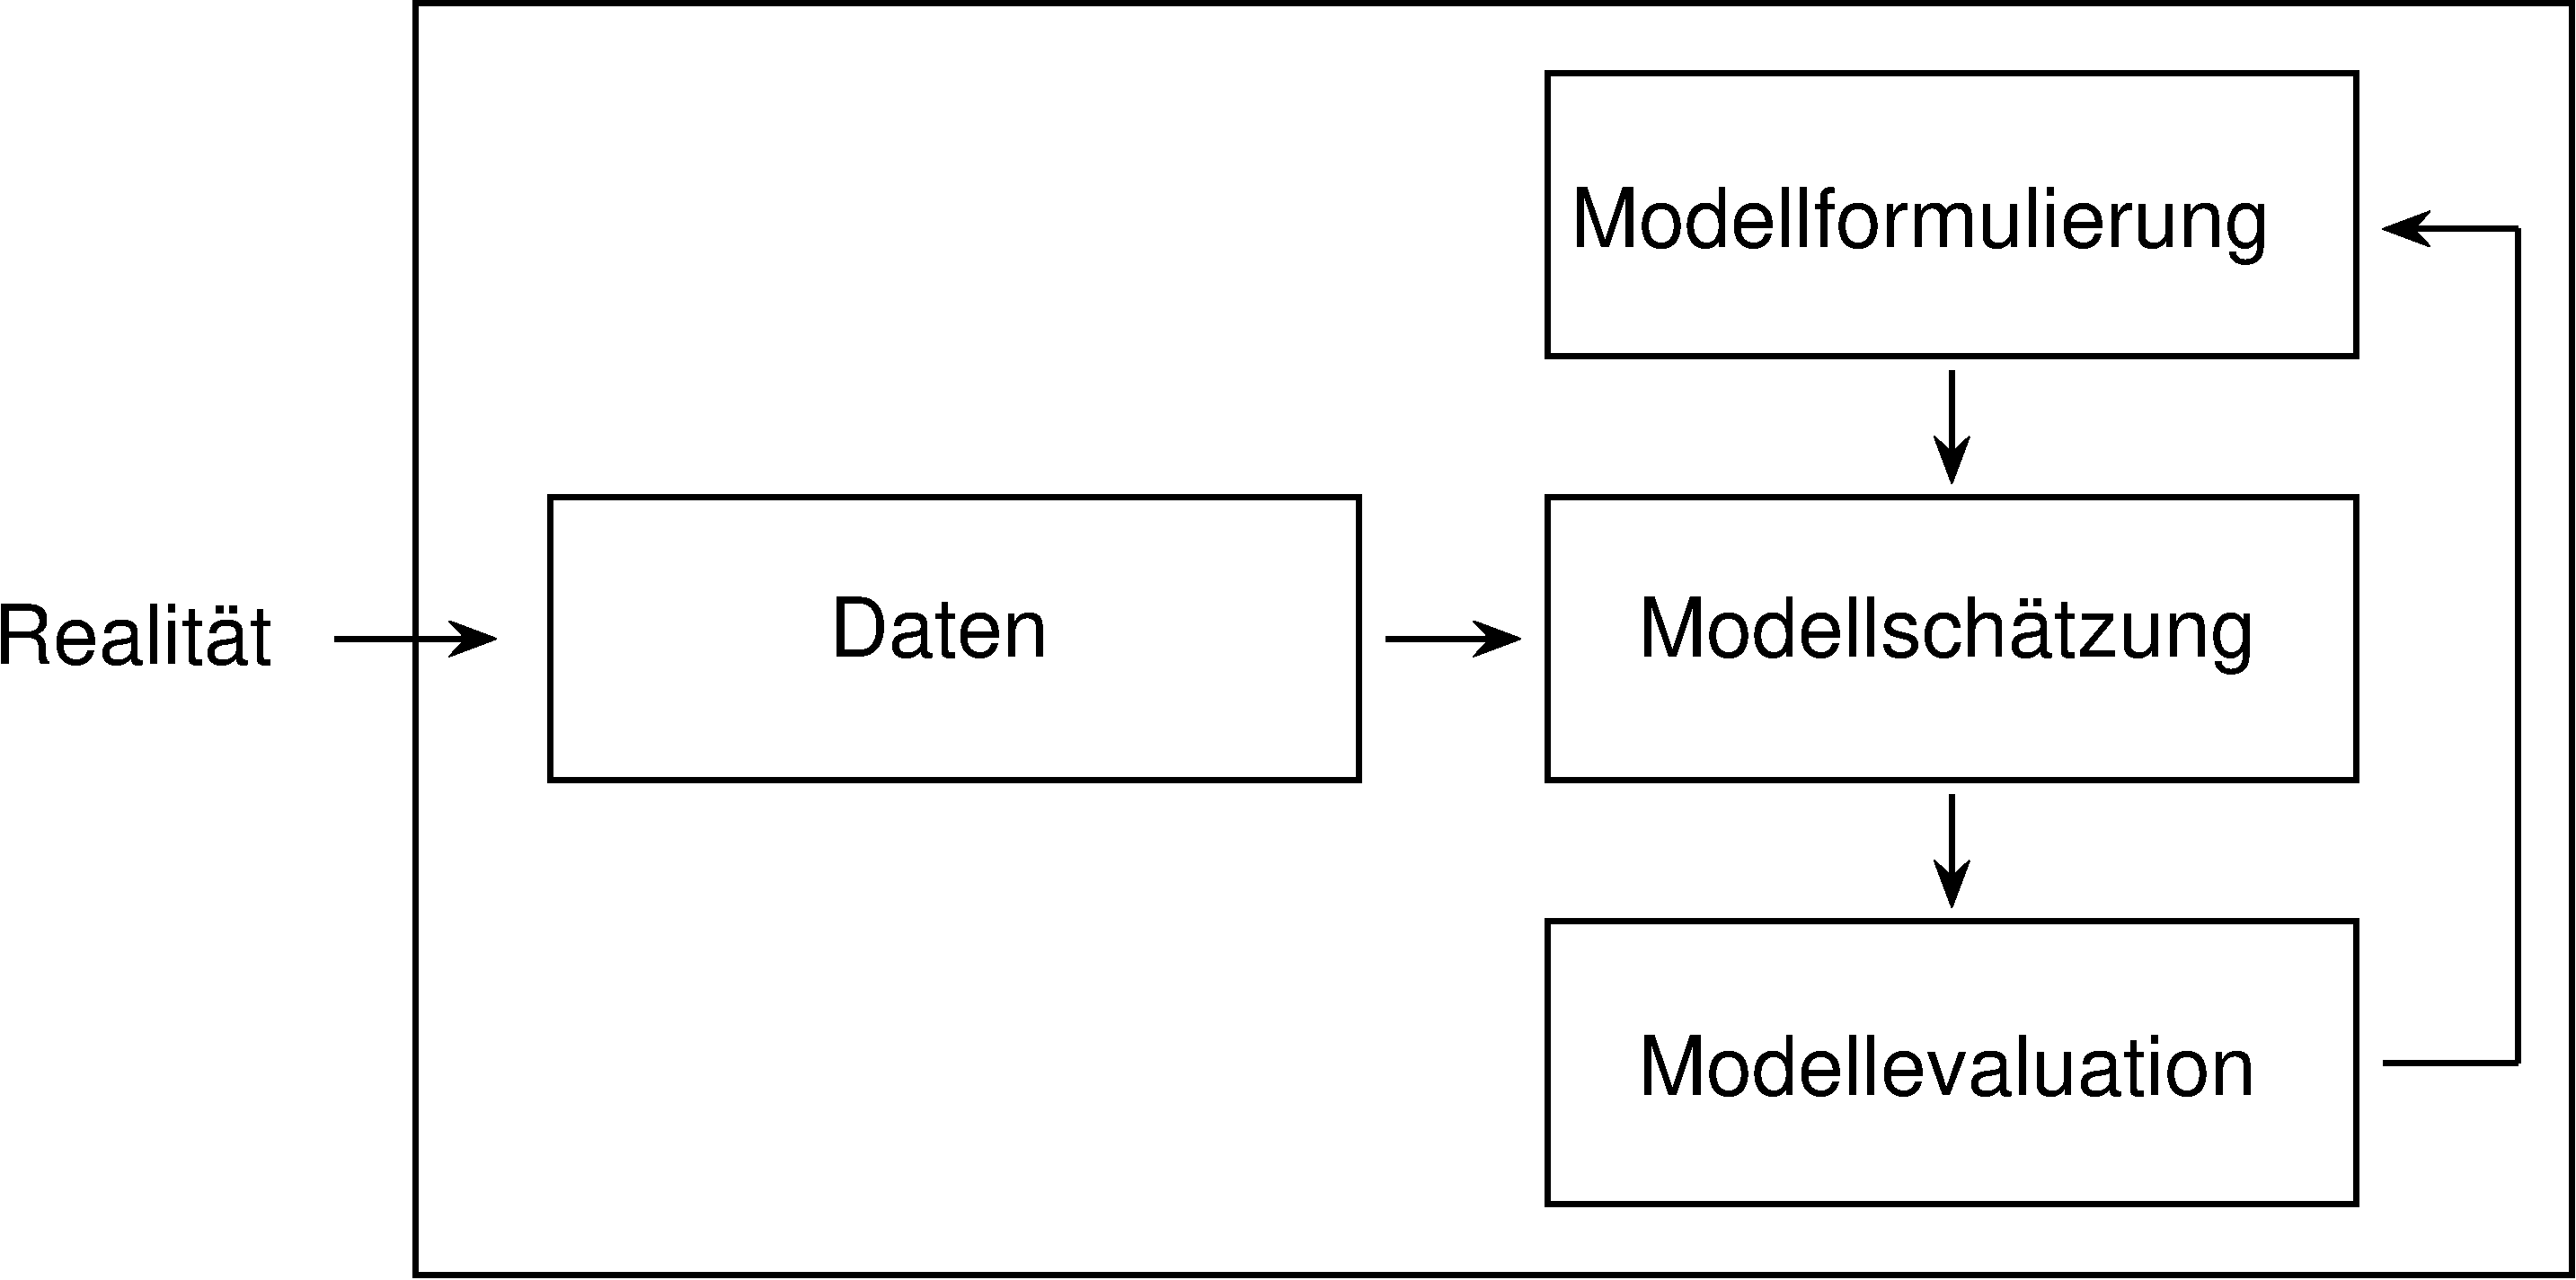
\includegraphics[width=0.9\linewidth]{7_Abbildungen/alm_7_wissenschaft} \end{center}
\end{frame}

\begin{frame}{}
\protect\hypertarget{section-3}{}
\vspace{1mm}
\normalsize

Modellformulierung \vspace{1mm} \small \begin{equation}
\upsilon = X\beta + \varepsilon, \varepsilon \sim N(0_n,\sigma^2I_n)
\end{equation} \vspace{5mm}

\normalsize

Modellschätzung \small \begin{equation}
\hat{\beta} = (X^TX)^{-1} X^T\upsilon,  \hat{\sigma}^2 = \frac{(\upsilon-X\hat{\beta})^T(\upsilon-X\hat{\beta})}{n-p}
\end{equation} \vspace{4mm}

\normalsize

Modellevaluation \small \begin{equation}
T = \frac{c^T\hat{\beta} - c^T\beta_0}{\sqrt{\hat{\sigma}^2c^T(X^TX)^{-1}c}},
F = \frac{(\hat{\varepsilon}_1^T\hat{\varepsilon}_1 - \hat{\varepsilon}^T\hat{\varepsilon})/p_2}{\hat{\varepsilon}^T\hat{\varepsilon}/(n-p)}
\end{equation}
\end{frame}

\begin{frame}{}
\protect\hypertarget{section-4}{}
Standardprobleme Frequentistischer Inferenz

\small
\vspace{2mm}

\noindent (1) Parameterschätzung

Ziel der Parameterschätzung ist es, einen möglichst guten Tipp für
wahre, aber unbekannte, Parameterwerte oder Funktionen dieser abzugeben,
typischerweise mithilfe von Daten.

\vspace{2mm}

\noindent (2) Konfidenzintervalle

Ziel der Bestimmung von Konfidenzintervallen ist es, basierend auf der
angenommenen Verteilung der Daten eine quantitative Aussage über die mit
Schätzwerten assoziierte Unsicherheit zu treffen.

\vspace{2mm}

\noindent (3) Hypothesentests

Ziel des Hypothesentestens ist es, basierend auf der angenommenen
Verteilung der Daten in einer möglichst zuverlässigen Form zu
entscheiden, ob ein wahrer, aber unbekannter Parameterwert in einer von
zwei sich gegenseitig ausschließenden Untermengen des Parameterraumes
liegt.
\end{frame}

\begin{frame}{}
\protect\hypertarget{section-5}{}
\center

\begin{center}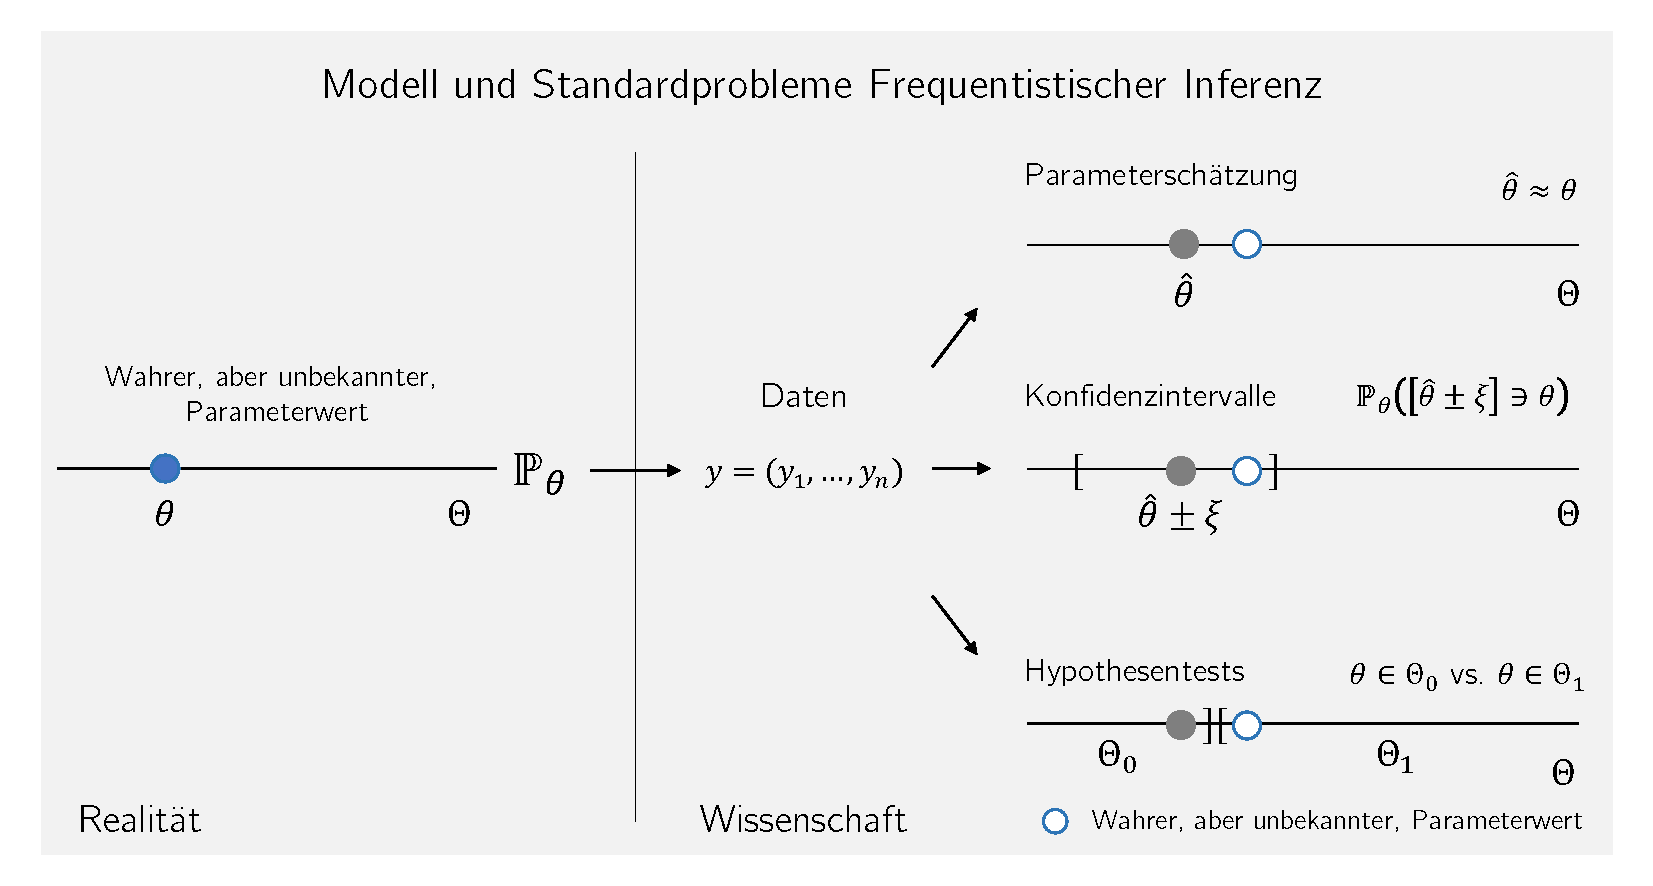
\includegraphics[width=1\linewidth]{7_Abbildungen/alm_7_frequentistische_inferenz} \end{center}
\center
\footnotesize

\(\theta := (\beta,\sigma^2)\),
\(\Theta := \mathbb{R}^p \times \mathbb{R}_{>0}\)
\(\mathbb{P}_\theta(y) := \mathbb{P}_{\beta,\sigma^2}(y)\) mit WDF
\(p_{\beta,\sigma^2}(\upsilon) := N(\upsilon;X\beta,\sigma^2I_n)\)
\end{frame}

\begin{frame}{}
\protect\hypertarget{section-6}{}
\small

Standardannahmen Frequentistischer Inferenz

\footnotesize
\setstretch{1.2}

Gegeben sei das Allgemeine Lineare Modell. Es wird angenommen, dass ein
vorliegender Datensatz eine der möglichen Realisierungen der Daten des
Modells ist. Aus Frequentistischer Sicht kann man unendlich oft
Datensätze basierend auf einem Modell generieren und zu jedem Datensatz
Schätzer oder Statistiken auswerten, z.B. den Betaparameterschätzer
\vspace{1mm}

\begin{itemize}
\item[] Datensatz (1) : $y^{(1)} = \left(y_1^{(1)}, y_2^{(1)}, ...,y_n^{(1)}\right)^T$  mit $\hat{\beta}^{(1)} = (X^TX)^{-1}X^Ty^{(1)}$
\item[] Datensatz (2) : $y^{(2)} = \left(y_1^{(2)}, y_2^{(2)}, ...,y_n^{(2)}\right)^T$  mit $\hat{\beta}^{(2)} = (X^TX)^{-1}X^Ty^{(2)}$
\item[] Datensatz (3) : $y^{(3)} = \left(y_1^{(3)}, y_2^{(3)}, ...,y_n^{(3)}\right)^T$  mit $\hat{\beta}^{(3)} = (X^TX)^{-1}X^Ty^{(3)}$
\item[] Datensatz (4) : $y^{(4)} = \left(y_1^{(4)}, y_2^{(4)}, ...,y_n^{(4)}\right)^T$  mit $\hat{\beta}^{(4)} = (X^TX)^{-1}X^Ty^{(4)}$
\item[] Datensatz (5) : $y^{(5)} = ...$
\end{itemize}

\vspace{1mm}

Um die Qualität statistischer Methoden zu beurteilen betrachtet die
Frequentistische Statistik die Wahrscheinlichkeitsverteilungen von
Schätzern und Statistiken unter Annahme der Datenverteilung. Was zum
Beispiel ist die Verteilung von \(\hat{\beta}^{(1)}\),
\(\hat{\beta}^{(2)}\), \(\hat{\beta}^{(3)}\), \(\hat{\beta}^{(4)}\),
\ldots{} also die Verteilung der Zufallsvariable
\(\hat{\beta} := (X^TX)^{-1}X^T\upsilon\)? Wenn eine statistische
Methode im Sinne der Frequentistischen Standardannahmen ``gut'' ist,
dann heißt das also, dass sie bei häufiger Anwendung ``im Mittel gut''
ist. Im Einzelfall, also im Normalfall nur eines vorliegenden
Datensatzes, kann sie auch ``schlecht'' sein.
\end{frame}

\begin{frame}{}
\protect\hypertarget{section-7}{}
Überblick

\small

\begin{itemize}
\item
  \justifying In diesem Abschnitt führen wir T-Statistiken als Maße zur
  Evaluation von Betaparameterschätzern im ALM ein. T-Statistiken
  quantifizieren dabei die geschätzten Effekte des
  Betaparameterschätzers in bezug zur durch den Varianzparameterschätzer
  geschätzten Residualvariabilität. Der Wert einer T-Statistik ist also
  zunächst einmal einfach als Signal-zu-Rauschen Verhältnis
  (Signal-to-Noise Ratio) zu verstehen.
\item
  \justifying T-Statistiken erlauben weiterhin die Evaluation von
  Linearkombinationen der Komponenten des Betaparameterschätzers im
  Sinne Frequentistischer Konfidenzinteralle und Hypothesentests. Wir
  betrachten hier zunächst nur die funktionale Form von T-Statistiken
  und ihre Frequentistische Verteilung zum Zwecke der
  Konfidenzintervallbestimmung. Der Einsatz von T-Teststatistiken im
  Rahmen von Einstich- und Zweistichproben T-Tests ist das Thema von
  Einheit (9) T-Tests.
\end{itemize}
\end{frame}

\begin{frame}{}
\protect\hypertarget{section-8}{}
\vfill
\large
\setstretch{3}

T-Zufallsvariablen

T-Statistiken

Konfidenzintervalle

Selbstkontrollfragen \vfill
\end{frame}

\begin{frame}{}
\protect\hypertarget{section-9}{}
\vfill
\large
\setstretch{3}

\textbf{T-Zufallsvariablen}

T-Statistiken

Konfidenzintervalle

Selbstkontrollfragen \vfill
\end{frame}

\begin{frame}{T-Zufallsvariablen}
\protect\hypertarget{t-zufallsvariablen}{}
\footnotesize
\begin{definition}[$t$-Zufallsvariable]
\justifying
$\xi$ sei eine Zufallsvariable mit Ergebnisraum $\mathbb{R}$ und WDF
\begin{equation}
p_\xi : \mathbb{R} \to \mathbb{R}_{>0}, x \mapsto p_\xi(x)
:= \frac{\Gamma\left(\frac{n+1}{2}\right)}{\sqrt{n\pi}\Gamma\left(\frac{n}{2}\right)}
\left(1 + \frac{x^2}{n} \right)^{-\frac{n+1}{2}},
\end{equation}
wobei $\Gamma$ die Gammafunktion bezeichne. Dann sagen wir, dass $\xi$ einer
$t$-Verteilung mit Freiheitsgradparameter $n$ unterliegt und nennen $\xi$ eine $t$-Zufallsvariable
mit Freiheitsgradparameter $n$. Wir kürzen dies mit $\xi \sim t(n)$ ab. Die WDF einer
$t$-Zufallsvariable bezeichnen wir mit $t(\cdot ;n)$. Die KVF und inverse KVF einer 
nichtzentralen $t$-Zufallsvariable bezeichnen wir mit $\Psi(\cdot;n)$ 
und $\Psi^{-1}(\cdot;n)$, respektive.
\end{definition}

Bemerkungen

\begin{itemize}
\tightlist
\item
  Die Verteilung ist um 0 symmetrisch
\item
  Steigendes \(n\) verschiebt Wahrscheinlichkeitsmasse aus den Ausläufen
  zum Zentrum.
\item
  Ab \(n = 30\) gilt \(t(n) \approx N(0,1)\).
\end{itemize}
\end{frame}

\begin{frame}{T-Zufallsvariablen}
\protect\hypertarget{t-zufallsvariablen-1}{}
\vfill

Wahrscheinlichkeitsdichtefunktionen von \(t\)-Zufallsvariablen
\vspace{5mm}

\begin{center}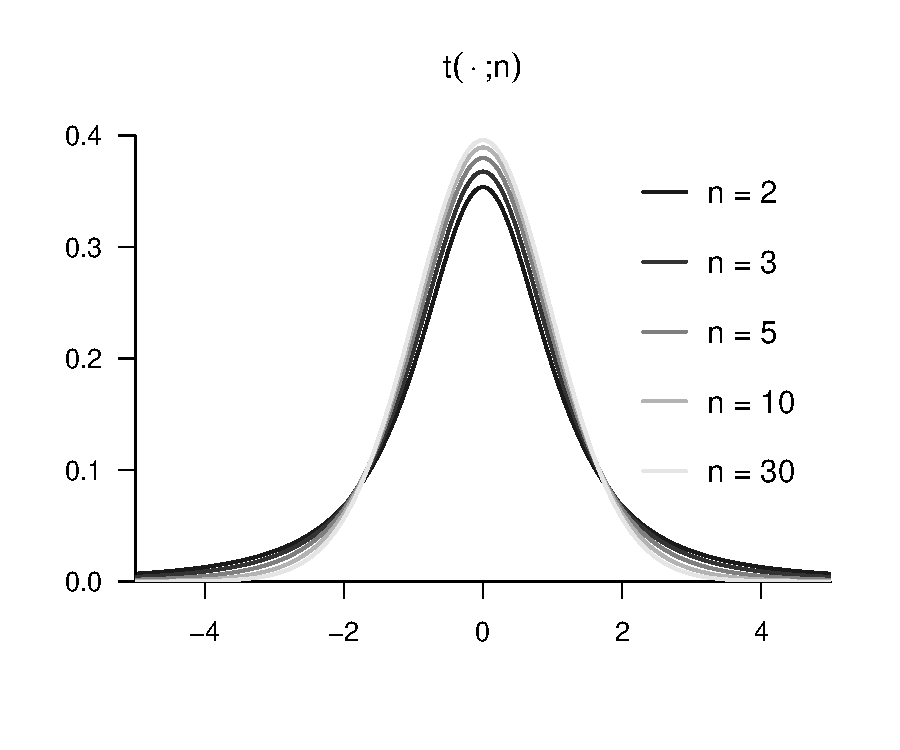
\includegraphics[width=0.7\linewidth]{7_Abbildungen/alm_7_t_wdf} \end{center}
\vspace{-3mm}
\footnotesize
\end{frame}

\begin{frame}{T-Zufallsvariablen}
\protect\hypertarget{t-zufallsvariablen-2}{}
\footnotesize
\begin{theorem}[$T$-Transformation]
\justifying
\normalfont
$Z \sim N(0,1)$ sei eine  $Z$-Zufallsvariable, $U \sim \chi^2(n)$ sei eine
$\chi^2$-Zufallsvariable Freiheitsgradparameter $n$, und $Z$ und $U$ seien
unabhängige Zufallsvariablen. Dann ist die Zufallsvariable
\begin{equation}
T := \frac{Z}{\sqrt{U/n}}
\end{equation}
eine $t$-verteilte Zufallsvariable mit Freiheitsgradparameter $n$, es gilt also $T \sim t(n)$.
\end{theorem}

Bemerkungen

\begin{itemize}
\tightlist
\item
  Das Theorem geht auf Student (1908) zurück.
\item
  Das Theorem ist eines der zentralen Resultate der Frequentistischen
  Statistik.
\item
  Zabell (2008) gibt hierzu einen historischen Überblick.
\end{itemize}
\end{frame}

\begin{frame}{T-Zufallsvariablen}
\protect\hypertarget{t-zufallsvariablen-3}{}
\footnotesize
\begin{definition}[Nichtzentrale $t$-Zufallsvariable]
\justifying
$\xi$ sei eine Zufallsvariable mit Ergebnisraum $\mathbb{R}$ und WDF
\begin{multline}
p_\xi : \mathbb{R} \to \mathbb{R}_{>0}, x \mapsto p_\xi(x) :=
\frac{1}{2^{\frac{n-1}{2}}\Gamma\left(\frac{n}{2} \right)(n \pi)^{\frac{1}{2}}} \\
\times \int_{0}^\infty \tau^{\frac{n-1}{2}} \exp\left(-\frac{\tau}{2}\right)
\exp\left(-\frac{1}{2}\left(x \left(\frac{\tau}{n}\right)^{\frac{1}{2}} - \delta \right)^2 \right)\,d\tau.
\end{multline}
Dann sagen wir, dass $\xi$ einer nichtzentralen $t$-Verteilung mit
Nichtzentralitätsparameter $\delta$ und Freiheitsgradparameter $n$ unterliegt
und nennen $\xi$ eine \textit{nichtzentrale $t$-Zufallsvariable mit Nichtzentralitätsparameter $\delta$ und
Freiheitsgradparameter $n$}. Wir kürzen dies mit $\xi \sim t(\delta, n)$ ab. Die WDF einer
nichtzentralen $t$-Zufallsvariable  bezeichnen wir mit
$t(\cdot;\delta,n)$. Die KVF und inverse KVF einer nichtzentralen $t$-Zufallsvariable
bezeichnen wir mit $\Psi(\cdot; \delta, n)$ und $\Psi^{-1}(\cdot; \delta, n)$, respektive.
\end{definition}

Bemerkungen

\begin{itemize}
\tightlist
\item
  Eine nichtzentrale \(t\)-Zufallsvariable mit \(\delta = 0\) ist eine
  \(t\)-Zufallsvariable.
\item
  Es gilt also \(t(\cdot;0,n) = t(\cdot;n)\).
\item
  Die funktionale Form der WDF findet sich zum Beispiel in Lehmann
  (1986), Seite 254, Gl. (80).
\end{itemize}
\end{frame}

\begin{frame}{T-Zufallsvariablen}
\protect\hypertarget{t-zufallsvariablen-4}{}
Wahrscheinlichkeitsdichtefunktionen nichtzentraler
\(t\)-Zufallsvariablen \vspace{4mm}

\begin{center}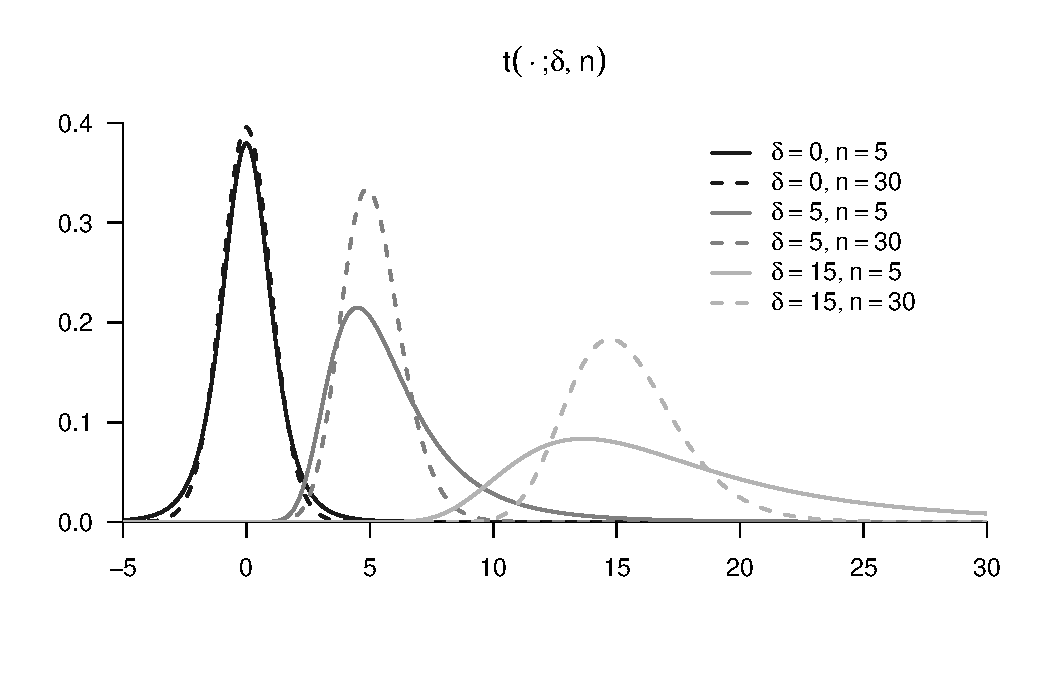
\includegraphics[width=0.9\linewidth]{7_Abbildungen/alm_7_nichtzentrale_t_verteilung} \end{center}
\end{frame}

\begin{frame}{T-Zufallsvariablen}
\protect\hypertarget{t-zufallsvariablen-5}{}
\footnotesize
\begin{theorem}[Nichtzentrale T-Transformation]
\normalfont
\justifying
$\xi \sim N(\mu,1)$ sei eine normalverteilte Zufallsvariable, $U \sim \chi^2(n)$
sei eine $\chi^2$ Zufallsvariable mit Freiheitsgradparameter $n$, und $\xi$ und
$U$ seien unabhängige Zufallsvariablen. Dann ist die Zufallsvariable
\begin{equation}
T := \frac{\xi}{\sqrt{U/n}}
\end{equation}
eine nichtzentrale $t$-Zufallsvariable mit Nichtzentralitätsparameter $\mu$ und
Freiheitsgradparameter $n$, es gilt also $T \sim t(\mu,n)$
\end{theorem}

Bemerkung

\begin{itemize}
\tightlist
\item
  Wir verzichten auf einen Beweis.
\end{itemize}
\end{frame}

\begin{frame}{}
\protect\hypertarget{section-10}{}
\vfill
\large
\setstretch{3}

T-Zufallsvariablen

\textbf{T-Statistiken}

Konfidenzintervalle

Selbstkontrollfragen \vfill
\end{frame}

\begin{frame}{T-Statistiken}
\protect\hypertarget{t-statistiken}{}
\footnotesize
\begin{definition}[T-Statistik]
Es sei 
\begin{equation}
\upsilon = X\beta + \varepsilon \mbox{ mit } \varepsilon \sim N\left(0_n,\sigma^2I_n\right) 
\end{equation}
das ALM. Weiterhin seien 
\begin{equation}
\hat{\beta} := (X^TX)^{-1}X^T\upsilon \mbox{ und } \hat{\sigma}^2 := \frac{(\upsilon - X\hat{\beta})^T(\upsilon - X\hat{\beta})}{n-p} 
\end{equation}
die Betaparameter- und Varianzparameterschätzer, respektive. Dann ist für einen 
\textit{Kontrastgewichtsvektor} $c \in \mathbb{R}^p$ und einen Parameter 
$\beta_0 \in \mathbb{R}^p$ die \textit{T-Statistik} definiert als 
\begin{equation}
T := \frac{c^T\hat{\beta} - c^T\beta_0}{\sqrt{\hat{\sigma}^2c^T(X^TX)^{-1}c}}. 
\end{equation}
\end{definition}

Bemerkungen

\begin{itemize}
\tightlist
\item
  Die T-Statistik hängt via \(\hat{\beta}\) und \(\hat{\sigma}^2\) von
  den Daten \(\upsilon\) ab.
\item
  Der Kontrastgewichtsvektor projiziert \(\hat{\beta}\) auf einen Skalar
  \(c^T\hat{\beta} \in \mathbb{R}\).
\item
  Die Wahl \(p\)-dimensionaler Einheitsvektoren für \(c\) erlaubt die
  Auswahl einzelner Komponenten von \(\hat{\beta}\) bzw. \(\beta_0\).
\item
  Eine generelle Wahl von \(c\) erlaubt die Evaluation beliebiger
  Linearkombinationen von \(\hat{\beta}\) bzw. \(\beta_0\).
\end{itemize}
\end{frame}

\begin{frame}{T-Statistiken}
\protect\hypertarget{t-statistiken-1}{}
\footnotesize

Bemerkungen (fortgeführt)

Die Wahl von \(\beta_0 \in \mathbb{R}^p\) erlaubt es, die T-Statistik
unterschiedlich einzusetzen:

\begin{itemize}
\item
  \justifying Wählt man \(\beta_0 := 0_p\), so erhält man mit der
  T-Statistik eine Deskriptivstatistik, die es erlaubt, geschätzte
  Regressoreffekte, also Komponenten oder Linearkombinationen von
  \(\hat{\beta}\), im Sinne eines Signal-zu-Rauschen Verhältnisses in
  Bezug zu der durch \(\hat{\sigma}^2\) quantifizierten
  Residualdatenvariabilität zu setzen. Der Nenner der T-Statistik stellt
  dabei sicher, dass insbesondere die adequate (Ko)Standardabweichung
  der entsprechenden Betaparameterkomponentenkombination als Bezugsgröße
  dient, da es sich bei \(\hat{\sigma}^2\left(X^TX\right)^{-1}\)
  bekanntlich um die Kovarianz des Betaparameterschätzers handelt.
  Folgende erste Intuition ist in diesem Kontext hilfreich:
  \begin{equation}
  T = \frac{\mbox{Geschätzte Effektstärke}}{\mbox{Geschätzte stichprobenumfangskalierte Datenvariabilität}}
  \end{equation}
\item
  \justifying Wählt man für \(\beta_0 = \beta\), also den wahren, aber
  unbekannten, Betaparameterwert, so eröffnet die T-Statistik die
  Möglichkeit, für einzelen Komponenten des Betaparametervektors
  Konfidenzintervalle zu bestimmen.
\item
  \justifying Deklariert man schließlich \(\beta_0 \in \Theta_0\) im
  Kontext eines Testszenarios als das Element einer Nullhypothese
  \(\Theta_0\), so eröffnet die T-Statistik die Hypothesentest-basierte
  Inferenz über Betaparameterkomponenten und ihrer Linearkombinationen.
  des ALMs.
\end{itemize}
\end{frame}

\begin{frame}{T-Statistiken}
\protect\hypertarget{t-statistiken-2}{}
\vspace{1mm}
\footnotesize
\begin{theorem}[T-Statistik]
\normalfont
\justifying
Es sei 
\begin{equation}
\upsilon = X\beta + \varepsilon \mbox{ mit } \varepsilon \sim N(0_n,\sigma^2I_n) 
\end{equation}
das ALM. Weiterhin seien 
\begin{equation}
\hat{\beta} := (X^TX)^{-1}X^T\upsilon \mbox{ und } \hat{\sigma}^2 := \frac{(\upsilon-X\hat{\beta})^T(\upsilon-X\hat{\beta})}{n-p} 
\end{equation}
die Betaparameter- und Varianzparameterschätzer, respektive. Schließlich sei für 
einen Kontrastgewichtsvektor $c \in \mathbb{R}^p$ und einen Parameter 
$\beta_0 \in \mathbb{R}^p$ 
\begin{equation}
T := \frac{c^T\hat{\beta} - c^T\beta_0}{\sqrt{\hat{\sigma}^2 c^T(X^TX)^{-1}c}}  
\end{equation}
die T-Statistik. Dann gilt 
\begin{equation}
T \sim t(\delta, n-p) \mbox{ mit } \delta := \frac{c^T\beta - c^T\beta_0}{\sqrt{\sigma^2 c^T(X^TX)^{-1}c}}. 
\end{equation}
\end{theorem}
\vspace{-2mm}

Bemerkungen \vspace{-2mm}

\begin{itemize}
\tightlist
\item
  Wir verzichten auf einen Beweis.
\item
  \(T\) ist eine Funktion der Parameterschätzer, \(\delta\) ist eine
  Funktion der wahren, aber unbekannten, Parameter
\item
  Für \(c^T\beta = c^T\beta_0\), also bei Zutreffen der Nullhypothese,
  gilt \(\delta = 0\) und damit \(T \sim t(n-p)\).
\item
  Für \(c^T\beta \neq c^T\beta_0\) kann die Verteilung von \(T\) zur
  Herleitung von Powerfunktionen benutzt werden.
\end{itemize}
\end{frame}

\begin{frame}{T-Statistiken}
\protect\hypertarget{t-statistiken-3}{}
Beispiel (1) Unabhängige und identisch normalverteilte Zufallsvariablen
\vspace{2mm} \footnotesize

Es sei \begin{equation}
\upsilon \sim N(X\beta,\sigma^2 I_n)
\mbox{ mit }
X := 1_n \in \mathbb{R}^{n\times 1},
\beta := \mu \in \mathbb{R}
\mbox{ und } \sigma^2 > 0.
\end{equation} das ALM Szenario unabhängiger und identisch
normalverteilter Zufallsvariablen und es seien \(c := 1\) und
\(\beta_0 := \mu_0\). Dann gilt für die T-Statistik \begin{equation}
T
= \frac{c^T\hat{\beta} - c^T\mu_0}{\sqrt{\hat{\sigma}^2c^T(X^TX)^{-1}c}}
= \frac{1^T\bar{\upsilon}- 1^T\mu_0}{\sqrt{s^2_y 1^T (1_n^T 1_n)^{-1}1}}
= \sqrt{n}\frac{\bar{\upsilon} - \mu_0}{s_\upsilon}
\end{equation} was der Einstichproben-T-Teststatistik für den Fall
\(\mu_0 = 0\) entspricht (vgl. Einheit (12) Hypothesentest in
Wahrscheinlichkeitstheorie und Frequentistische Inferenz und Einheit (9)
T-Tests in Allgemeines Lineares Modell). Die hier betrachtete
T-Statistik nimmt hohe Werte für hohe Werte von \(\bar{\upsilon}\)
(Effekt), kleine Werte von \(s_\upsilon^2\) (Datenvariabilität) und hohe
Werte von \(n\) (Stichprobenumfang) an.

Eine beliebte Definition in diesem Zusammenhang ist \textit{Cohen's $d$}
als \textit{Effektstärkenmaß}. Es gilt \begin{equation}
d := \frac{\bar{\upsilon}}{s_\upsilon},
\end{equation} so dass für \(\mu_0 := 0\) gilt, dass \begin{equation}
T = \sqrt{n}d \mbox{ bzw. } d = \frac{1}{\sqrt{n}} T.
\end{equation} Cohen's \(d\) ist also ein stichprobenumfangunabhängiges
Signal-zu-Rauschen Verhältnis.
\end{frame}

\begin{frame}[fragile]{T-Statistiken}
\protect\hypertarget{t-statistiken-4}{}
Simulation (1) Unabhängig und identische normalverteilte
Zufallsvariablen

\small

Wahre, aber unbekannte, Hypothesenszenarien \(c^T\beta = c^T\beta_0\)
und \(c^T\beta \neq c^T\beta_0\)

\vspace{2mm}
\tiny
\setstretch{1}

\begin{Shaded}
\begin{Highlighting}[]
\CommentTok{\# Libraries}
\FunctionTok{library}\NormalTok{(MASS)                                                  }\CommentTok{\# multivariate Normalverteilung}

\CommentTok{\# Modellformulierung}
\NormalTok{n          }\OtherTok{=} \DecValTok{12}                                                \CommentTok{\# Anzahl von Datenpunkten}
\NormalTok{p          }\OtherTok{=} \DecValTok{1}                                                 \CommentTok{\# Anzahl von Betaparametern}
\NormalTok{X          }\OtherTok{=} \FunctionTok{matrix}\NormalTok{(}\FunctionTok{c}\NormalTok{(}\FunctionTok{rep}\NormalTok{(}\DecValTok{1}\NormalTok{,n)), }\AttributeTok{nrow =}\NormalTok{ n)                     }\CommentTok{\# Designmatrix}
\NormalTok{I\_n        }\OtherTok{=} \FunctionTok{diag}\NormalTok{(n)                                           }\CommentTok{\# Einheitsmatrix}
\NormalTok{beta       }\OtherTok{=} \FunctionTok{c}\NormalTok{(}\DecValTok{0}\NormalTok{,}\DecValTok{1}\NormalTok{)                                            }\CommentTok{\# wahre , aber unbekannte , Betaparameter}
\NormalTok{nscn       }\OtherTok{=} \FunctionTok{length}\NormalTok{(beta)                                      }\CommentTok{\# Anzahl wahrer, aber unbekannter, Hypothesenszenarien}
\NormalTok{sigsqr     }\OtherTok{=} \DecValTok{1}                                                 \CommentTok{\# wahrer, aber unbekannter, Varianzparameter}
\NormalTok{c          }\OtherTok{=} \DecValTok{1}                                                 \CommentTok{\# Kontrastvektor von Interessse}
\NormalTok{beta\_0     }\OtherTok{=} \DecValTok{0}                                                 \CommentTok{\# Nullhypothesenbetaparameter}

\CommentTok{\# Frequentistische Simulation}
\NormalTok{nsim       }\OtherTok{=} \FloatTok{1e4}                                               \CommentTok{\# Anzahl Simulationen}
\NormalTok{delta      }\OtherTok{=} \FunctionTok{rep}\NormalTok{(}\ConstantTok{NaN}\NormalTok{, nscn)                                    }\CommentTok{\# Anzahl Nichtzentralitätsparameter}
\NormalTok{Tee        }\OtherTok{=} \FunctionTok{matrix}\NormalTok{(}\FunctionTok{rep}\NormalTok{(}\ConstantTok{NaN}\NormalTok{, nscn}\SpecialCharTok{*}\NormalTok{nsim), }\AttributeTok{ncol =}\NormalTok{ nscn)          }\CommentTok{\# T{-}Teststatistik Realisierungsarray}
\ControlFlowTok{for}\NormalTok{(s }\ControlFlowTok{in} \DecValTok{1}\SpecialCharTok{:}\NormalTok{nscn)\{                                              }\CommentTok{\# Hypothesenszenarien}
\NormalTok{  delta[s]    }\OtherTok{=}\NormalTok{ ((}\FunctionTok{t}\NormalTok{(c) }\SpecialCharTok{\%*\%}\NormalTok{ beta[s] }\SpecialCharTok{{-}} \FunctionTok{t}\NormalTok{(c) }\SpecialCharTok{\%*\%}\NormalTok{ beta\_0)}\SpecialCharTok{/}         \CommentTok{\# Nichtzentralitätsparameter}
                \FunctionTok{sqrt}\NormalTok{(sigsqr}\SpecialCharTok{*}\FunctionTok{t}\NormalTok{(c)}\SpecialCharTok{\%*\%}\FunctionTok{solve}\NormalTok{(}\FunctionTok{t}\NormalTok{(X)}\SpecialCharTok{\%*\%}\NormalTok{X)}\SpecialCharTok{\%*\%}\NormalTok{c))}
  \ControlFlowTok{for}\NormalTok{(i }\ControlFlowTok{in} \DecValTok{1}\SpecialCharTok{:}\NormalTok{nsim)\{                                            }\CommentTok{\# Simulationsiterationen}
\NormalTok{    y          }\OtherTok{=} \FunctionTok{mvrnorm}\NormalTok{(}\DecValTok{1}\NormalTok{, X }\SpecialCharTok{\%*\%}\NormalTok{ beta[s], sigsqr}\SpecialCharTok{*}\NormalTok{I\_n)         }\CommentTok{\# y}
\NormalTok{    beta\_hat   }\OtherTok{=} \FunctionTok{solve}\NormalTok{(}\FunctionTok{t}\NormalTok{(X) }\SpecialCharTok{\%*\%}\NormalTok{ X) }\SpecialCharTok{\%*\%} \FunctionTok{t}\NormalTok{(X) }\SpecialCharTok{\%*\%}\NormalTok{ y              }\CommentTok{\# \textbackslash{}hat\{\textbackslash{}beta\}}
\NormalTok{    eps\_hat    }\OtherTok{=}\NormalTok{ y }\SpecialCharTok{{-}}\NormalTok{ X }\SpecialCharTok{\%*\%}\NormalTok{ beta\_hat                            }\CommentTok{\# \textbackslash{}hat\{\textbackslash{}eps\}}
\NormalTok{    sigsqr\_hat }\OtherTok{=}\NormalTok{ (}\FunctionTok{t}\NormalTok{(eps\_hat) }\SpecialCharTok{\%*\%}\NormalTok{ eps\_hat)}\SpecialCharTok{/}\NormalTok{(n}\SpecialCharTok{{-}}\NormalTok{p)                }\CommentTok{\# \textbackslash{}hat\{\textbackslash{}sigma\}\^{}2}
\NormalTok{    Tee[i,s]   }\OtherTok{=}\NormalTok{ ((}\FunctionTok{t}\NormalTok{(c) }\SpecialCharTok{\%*\%}\NormalTok{ beta\_hat }\SpecialCharTok{{-}} \FunctionTok{t}\NormalTok{(c) }\SpecialCharTok{\%*\%}\NormalTok{ beta\_0)}\SpecialCharTok{/}       \CommentTok{\# T}
                  \FunctionTok{sqrt}\NormalTok{(sigsqr\_hat}\SpecialCharTok{*}\FunctionTok{t}\NormalTok{(c)}\SpecialCharTok{\%*\%}\FunctionTok{solve}\NormalTok{(}\FunctionTok{t}\NormalTok{(X)}\SpecialCharTok{\%*\%}\NormalTok{X)}\SpecialCharTok{\%*\%}\NormalTok{c))}
\NormalTok{  \}}
\NormalTok{\}}
\end{Highlighting}
\end{Shaded}
\end{frame}

\begin{frame}{T-Statistiken}
\protect\hypertarget{t-statistiken-5}{}
Simulation (1) Unabhängig und identische normalverteilte
Zufallsvariablen

\footnotesize

Wahre, aber unbekannte, Hypothesenszenarien \(c^T\beta = c^T\beta_0\)
und \(c^T\beta \neq c^T\beta_0\)

\vspace{8mm}

\begin{center}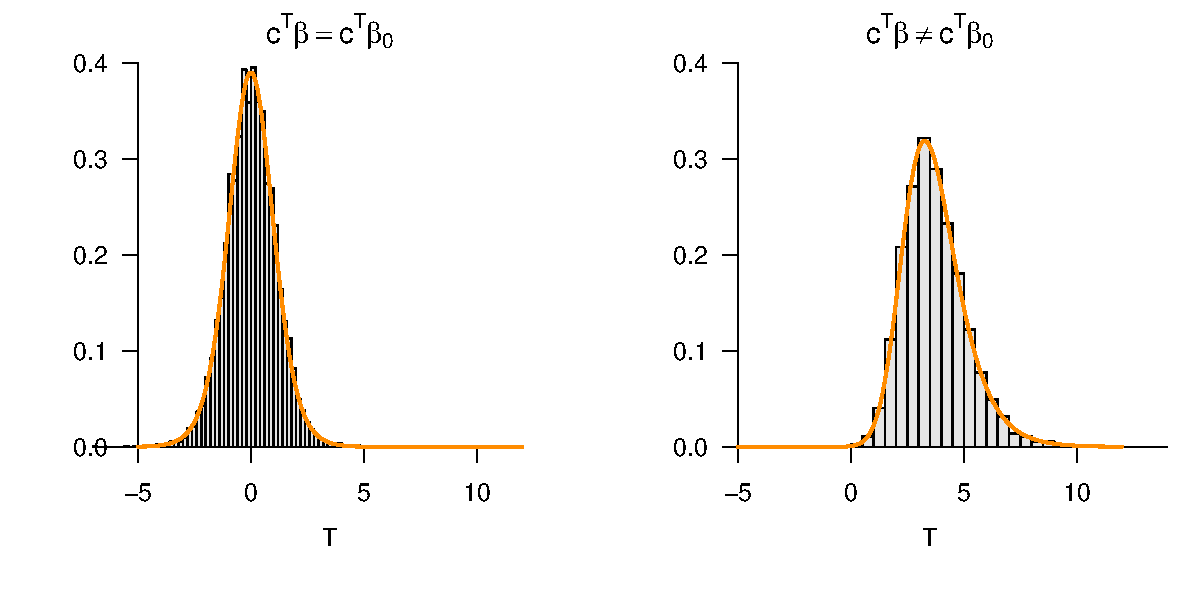
\includegraphics[width=1\linewidth]{7_Abbildungen/alm_7_T_Teststatistik_1} \end{center}
\end{frame}

\begin{frame}[fragile]{T-Statistiken}
\protect\hypertarget{t-statistiken-6}{}
Simulation (1) Einfache lineare Regression

\small

Wahre, aber unbekannte, Hypothesenszenarien \(c^T\beta = c^T\beta_0\)
und \(c^T\beta \neq c^T\beta_0\)

\vspace{2mm}
\tiny
\setstretch{1}

\begin{Shaded}
\begin{Highlighting}[]
\CommentTok{\# Modellformulierung}
\FunctionTok{library}\NormalTok{(MASS)                                                  }\CommentTok{\# multivariate Normalverteilung}
\NormalTok{n          }\OtherTok{=} \DecValTok{10}                                                \CommentTok{\# Anzahl von Datenpunkten}
\NormalTok{p          }\OtherTok{=} \DecValTok{2}                                                 \CommentTok{\# Anzahl von Betaparametern}
\NormalTok{x          }\OtherTok{=} \DecValTok{1}\SpecialCharTok{:}\NormalTok{n                                               }\CommentTok{\# Prädiktorwerte}
\NormalTok{X          }\OtherTok{=} \FunctionTok{matrix}\NormalTok{(}\FunctionTok{c}\NormalTok{(}\FunctionTok{rep}\NormalTok{(}\DecValTok{1}\NormalTok{,n),x), }\AttributeTok{ncol =}\NormalTok{ p)                   }\CommentTok{\# Designmatrix}
\NormalTok{I\_n        }\OtherTok{=} \FunctionTok{diag}\NormalTok{(n)                                           }\CommentTok{\# Einheitsmatrix}
\NormalTok{beta       }\OtherTok{=} \FunctionTok{matrix}\NormalTok{(}\FunctionTok{c}\NormalTok{(}\DecValTok{1}\NormalTok{,}\DecValTok{0}\NormalTok{,}\DecValTok{1}\NormalTok{,}\DecValTok{1}\NormalTok{), }\AttributeTok{nrow =} \DecValTok{2}\NormalTok{)                      }\CommentTok{\# wahre , aber unbekannte , Betaparameter}
\NormalTok{nscn       }\OtherTok{=} \FunctionTok{ncol}\NormalTok{(beta)                                        }\CommentTok{\# Anzahl wahrer, aber unbekannter, Hypothesenszenarien}
\NormalTok{sigsqr     }\OtherTok{=} \DecValTok{1}                                                 \CommentTok{\# wahrer, aber unbekannter, Varianzparameter}
\NormalTok{c          }\OtherTok{=} \FunctionTok{matrix}\NormalTok{(}\FunctionTok{c}\NormalTok{(}\DecValTok{0}\NormalTok{,}\DecValTok{1}\NormalTok{), }\AttributeTok{nrow =} \DecValTok{2}\NormalTok{)                          }\CommentTok{\# Kontrastvektor von Interessse}
\NormalTok{beta\_0     }\OtherTok{=} \FunctionTok{matrix}\NormalTok{(}\FunctionTok{c}\NormalTok{(}\DecValTok{0}\NormalTok{,}\DecValTok{0}\NormalTok{), }\AttributeTok{nrow =} \DecValTok{2}\NormalTok{)                          }\CommentTok{\# Nullhypothesenbetaparameter}

\CommentTok{\# Frequentistische Simulation}
\NormalTok{nsim       }\OtherTok{=} \FloatTok{1e4}                                               \CommentTok{\# Anzahl Simulationen}
\NormalTok{delta      }\OtherTok{=} \FunctionTok{rep}\NormalTok{(}\ConstantTok{NaN}\NormalTok{, nscn)                                    }\CommentTok{\# Anzahl Nichtzentralitätsparameter}
\NormalTok{Tee        }\OtherTok{=} \FunctionTok{matrix}\NormalTok{(}\FunctionTok{rep}\NormalTok{(}\ConstantTok{NaN}\NormalTok{, nscn}\SpecialCharTok{*}\NormalTok{nsim), }\AttributeTok{ncol =}\NormalTok{ nscn)          }\CommentTok{\# T{-}Teststatistik Realisierungsarray}
\ControlFlowTok{for}\NormalTok{(s }\ControlFlowTok{in} \DecValTok{1}\SpecialCharTok{:}\NormalTok{nscn)\{                                              }\CommentTok{\# Hypothesenszenarien}
\NormalTok{  delta[s]    }\OtherTok{=}\NormalTok{ ((}\FunctionTok{t}\NormalTok{(c) }\SpecialCharTok{\%*\%}\NormalTok{ beta[,s] }\SpecialCharTok{{-}} \FunctionTok{t}\NormalTok{(c) }\SpecialCharTok{\%*\%}\NormalTok{ beta\_0)}\SpecialCharTok{/}        \CommentTok{\# Nichtzentralitätsparameter}
                \FunctionTok{sqrt}\NormalTok{(sigsqr}\SpecialCharTok{*}\FunctionTok{t}\NormalTok{(c)}\SpecialCharTok{\%*\%}\FunctionTok{solve}\NormalTok{(}\FunctionTok{t}\NormalTok{(X)}\SpecialCharTok{\%*\%}\NormalTok{X)}\SpecialCharTok{\%*\%}\NormalTok{c))}
  \ControlFlowTok{for}\NormalTok{(i }\ControlFlowTok{in} \DecValTok{1}\SpecialCharTok{:}\NormalTok{nsim)\{                                            }\CommentTok{\# Simulationsiterationen}
\NormalTok{    y          }\OtherTok{=} \FunctionTok{mvrnorm}\NormalTok{(}\DecValTok{1}\NormalTok{, X }\SpecialCharTok{\%*\%}\NormalTok{ beta[,s], sigsqr}\SpecialCharTok{*}\NormalTok{I\_n)        }\CommentTok{\# y}
\NormalTok{    beta\_hat   }\OtherTok{=} \FunctionTok{solve}\NormalTok{(}\FunctionTok{t}\NormalTok{(X) }\SpecialCharTok{\%*\%}\NormalTok{ X) }\SpecialCharTok{\%*\%} \FunctionTok{t}\NormalTok{(X) }\SpecialCharTok{\%*\%}\NormalTok{ y              }\CommentTok{\# \textbackslash{}hat\{\textbackslash{}beta\}}
\NormalTok{    eps\_hat    }\OtherTok{=}\NormalTok{ y }\SpecialCharTok{{-}}\NormalTok{ X }\SpecialCharTok{\%*\%}\NormalTok{ beta\_hat                            }\CommentTok{\# \textbackslash{}hat\{\textbackslash{}eps\}}
\NormalTok{    sigsqr\_hat }\OtherTok{=}\NormalTok{ (}\FunctionTok{t}\NormalTok{(eps\_hat) }\SpecialCharTok{\%*\%}\NormalTok{ eps\_hat)}\SpecialCharTok{/}\NormalTok{(n}\SpecialCharTok{{-}}\NormalTok{p)                }\CommentTok{\# \textbackslash{}hat\{\textbackslash{}sigma\}\^{}2}
\NormalTok{    Tee[i,s]   }\OtherTok{=}\NormalTok{ ((}\FunctionTok{t}\NormalTok{(c) }\SpecialCharTok{\%*\%}\NormalTok{ beta\_hat }\SpecialCharTok{{-}} \FunctionTok{t}\NormalTok{(c) }\SpecialCharTok{\%*\%}\NormalTok{ beta\_0)}\SpecialCharTok{/}       \CommentTok{\# T}
                  \FunctionTok{sqrt}\NormalTok{(sigsqr\_hat}\SpecialCharTok{*}\FunctionTok{t}\NormalTok{(c)}\SpecialCharTok{\%*\%}\FunctionTok{solve}\NormalTok{(}\FunctionTok{t}\NormalTok{(X)}\SpecialCharTok{\%*\%}\NormalTok{X)}\SpecialCharTok{\%*\%}\NormalTok{c))}
\NormalTok{  \}}
\NormalTok{\}}
\end{Highlighting}
\end{Shaded}
\end{frame}

\begin{frame}{T-Statistiken}
\protect\hypertarget{t-statistiken-7}{}
Simulation (1) Einfache lineare Regression

\small

Wahre, aber unbekannte, Hypothesenszenarien \(c^T\beta = c^T\beta_0\)
und \(c^T\beta \neq c^T\beta_0\)

\vspace{8mm}

\begin{center}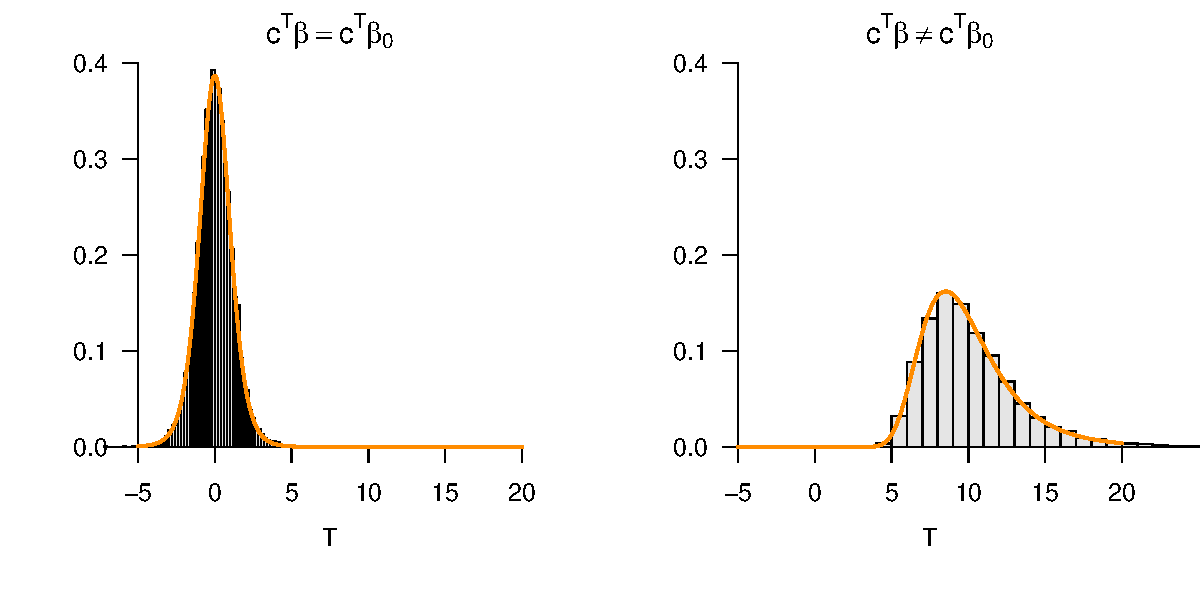
\includegraphics[width=1\linewidth]{7_Abbildungen/alm_7_T_Teststatistik_2} \end{center}
\end{frame}

\begin{frame}{}
\protect\hypertarget{section-11}{}
\vfill
\large
\setstretch{3}

T-Zufallsvariablen

T-Statistiken

\textbf{Konfidenzintervalle}

Selbstkontrollfragen \vfill
\end{frame}

\begin{frame}{Konfidenzintervalle}
\protect\hypertarget{konfidenzintervalle}{}
\footnotesize
\begin{theorem}[Konfidenzintervalle für Betaparameterkomponenten]
\justifying
\normalfont
Es sei
\begin{equation}
\upsilon = X\beta + \varepsilon \mbox{ mit } \varepsilon \sim N(0_n,\sigma^2I_n)
\end{equation}
das ALM,  $\hat{\beta}$ und $\hat{\sigma}^2$ seien die Betaparameter- und Varianzparameterschätzer,
respektive und und für ein $\delta \in ]0,1[$ sei 
\begin{equation}
t_\delta := \Psi^{-1}\left(\frac{1+\delta}{2}; n - p \right).
\end{equation}
Schließlich sei für $j = 1,...p$
\begin{equation}
\lambda_j := \left(\left(X^TX \right)^{-1}\right)_{jj}
\mbox{ das $j$te Diagonalelement von } \left(X^TX \right)^{-1}. 
\end{equation}
Dann ist für $j = 1,...p$
\begin{equation}
\kappa_j := \left[\hat{\beta}_j - \hat{\sigma}\sqrt{\lambda_j}t_{\delta},\hat{\beta}_j + \hat{\sigma}\sqrt{\lambda_j}t_{\delta}\right]
\end{equation}
ein $\delta$-Konfidenzintervall für die $j$te Komponente $\beta_j$ des Betaparameters $\beta = (\beta_1,...,\beta_p)^T$.
\end{theorem}

Bemerkungen

\begin{itemize}
\tightlist
\item
  Intuitiv gilt im Vergleich zum Konfidenzintervall für den
  Erwartungswertparameter bei Normalverteilung \begin{equation}
  \hat{\beta}_j \approx \bar{\upsilon}, \hat{\sigma} \approx S, \sqrt{\lambda_j} \approx \sqrt{n^{-1}} \mbox{ und } t_\delta = t_\delta,
  \end{equation} vgl. (11) Konfidenzintervalle in
  Wahrscheinlichkeitstheorie und Frequentistische Inferenz.
\end{itemize}
\end{frame}

\begin{frame}{Konfidenzintervalle}
\protect\hypertarget{konfidenzintervalle-1}{}
\footnotesize

\underline{Beweis}

Wir müssen zeigen, dass \begin{equation}
\mathbb{P}(\kappa_j \ni \beta_j) = \delta.
\end{equation} Dazu halten wir zunächst fest, dass für alle
\(j = 1,...,p\) bei Wahl von \(\beta_0 = \beta\) und \(c := e_j\) nach
dem Theorem zur T-Statistik für \(T \sim t(\delta,n-p)\) gilt, dass
\begin{align}
\begin{split}
T 
= \frac{e_j^T\hat{\beta} - e_j^T\beta}{\sqrt{\hat{\sigma}^2e_j^T\left(X^TX\right)^{-1}e_j}} 
= \frac{\hat{\beta}_j - \beta_j}{\sqrt{\hat{\sigma}^2 \left(\left(X^TX \right)^{-1}\right)_{jj}}}
= \frac{\hat{\beta}_j - \beta_j}{\hat{\sigma} \sqrt{\lambda_j}}
=: T_j.
\end{split}
\end{align} und \begin{align}
\begin{split}
\delta
= \frac{e_j\beta - e_j^T\beta}{\sqrt{\hat{\sigma}^2e_j^T\left(X^TX\right)^{-1}e_j}} 
= 0
\end{split}
\end{align} Damit gilt dann auch sofort, dass \(T_j \sim t(n-p)\).
Weiterhin erinnern erinnern wir daran (vgl. (11) Konfidenzintervalle in
Wahrscheinlichkeitstheorie und Frequentistischer Inferenz), dass per
Definition von \(t_\delta\) gilt, dass \begin{equation}
\mathbb{P}\left(-t_\delta \le T_j \le t_\delta \right)
\end{equation}
\end{frame}

\begin{frame}{Konfidenzintervalle}
\protect\hypertarget{konfidenzintervalle-2}{}
\footnotesize

\underline{Beweis (fortgeführt)}

Aus der Definition eines \(\delta\)-Konfidenzintervalls folgt dann
\begin{align}
\begin{split}
\delta 
& = \mathbb{P}\left(-t_\delta \le T_j \le t_\delta \right) \\
& = \mathbb{P}\left(-t_\delta \le \frac{\hat{\beta}_j - \beta_j}{\hat{\sigma}\sqrt{\lambda_j}} \le t_\delta \right) \\
& = \mathbb{P}\left(-t_\delta\hat{\sigma}\sqrt{\lambda_j} \le \hat{\beta}_j - \beta_j \le t_\delta\hat{\sigma}\sqrt{\lambda_j} \right) \\
& = \mathbb{P}\left(-\hat{\beta}_j -t_\delta\hat{\sigma}\sqrt{\lambda_j} \le - \beta_j \le -\hat{\beta}_j + t_\delta\hat{\sigma}\sqrt{\lambda_j} \right) \\
& = \mathbb{P}\left(\hat{\beta}_j + t_\delta\hat{\sigma}\sqrt{\lambda_j} \ge \beta_j \ge \hat{\beta}_j - t_\delta\hat{\sigma}\sqrt{\lambda_j} \right) \\
& = \mathbb{P}\left(\hat{\beta}_j - t_\delta\hat{\sigma}\sqrt{\lambda_j}  \le \beta_j \le \hat{\beta}_j + t_\delta\hat{\sigma}\sqrt{\lambda_j} \right) \\
& = \mathbb{P}\left(\left[\hat{\beta}_j - \hat{\sigma}\sqrt{\lambda_j}t_{\delta},\hat{\beta}_j + \hat{\sigma}\sqrt{\lambda_j}t_{\delta}\right]  \ni \beta_j \right) \\
& = \mathbb{P}(\kappa_j \ni \beta_j) 
\end{split}
\end{align} und damit ist alles gezeigt.
\end{frame}

\begin{frame}{Konfidenzintervalle}
\protect\hypertarget{konfidenzintervalle-3}{}
Konfidenzintervall bei unabhängigen und identische normalverteilten
Zufallsvariablen

\footnotesize

Wir betrachten die ALM Form des Szenarios unabhängig und identisch
normalverteilter Zufallsvariablen

\begin{equation}
\upsilon \sim N(X\beta,\sigma^2I_n) \mbox{ mit }  X := 1_{n} \in \mathbb{R}^n, \beta := \mu \in \mathbb{R},\sigma^2 > 0
\end{equation} Dann gelten, wie bereits gesehen \begin{equation}
\hat{\beta} = \frac{1}{n}\sum_{i=1}^n \upsilon_i =: \bar{\upsilon},
\hat{\sigma}^2 = \frac{1}{n-1}\sum_{i=1}^n(\upsilon_i-\bar{\upsilon})^2 =: s^2 \mbox{ und }
\lambda_1 = \left(1_n^T1_n\right)^{-1} = \frac{1}{n}
\end{equation} Nach dem Theorem zu Konfidenzintervallen für
Betaparameterkomponenten gilt dann, dass \begin{equation}
\kappa := \left[\bar{\upsilon} - \frac{s}{\sqrt{n}}t_{\delta}, \bar{\upsilon} + \frac{s}{\sqrt{n}}t_{\delta}\right]
\end{equation} ein \(\delta\)-Konfidenzintervall für \(\beta\) ist und
dieses ist offenbar identisch mit dem \(\delta\)-Konfidenzintervall für
den Erwartungsparameter der Normalverteilung, welches wir in (9)
Konfidenzintervalle in Wahrscheinlichkeitstheorie und Frequentistische
Inferenz eingeführt haben.
\end{frame}

\begin{frame}[fragile]{Konfidenzintervalle}
\protect\hypertarget{konfidenzintervalle-4}{}
Simulation von Konfidenzintervallen bei einfacher linearer Regression

\vspace{1mm}
\setstretch{1.1}
\tiny

\begin{Shaded}
\begin{Highlighting}[]
\CommentTok{\# Modellformulierung}
\FunctionTok{library}\NormalTok{(MASS)                                                       }\CommentTok{\# multivariate Normalverteilung}
\FunctionTok{set.seed}\NormalTok{(}\DecValTok{0}\NormalTok{)                                                         }\CommentTok{\# random number generator seed}
\NormalTok{ns         }\OtherTok{=} \FloatTok{1e2}                                                    \CommentTok{\# Anzahl Simulationen}
\NormalTok{n          }\OtherTok{=} \DecValTok{10}                                                     \CommentTok{\# Anzahl von Datenpunkten}
\NormalTok{p          }\OtherTok{=} \DecValTok{2}                                                      \CommentTok{\# Anzahl von Betaparametern}
\NormalTok{x          }\OtherTok{=} \DecValTok{1}\SpecialCharTok{:}\NormalTok{n                                                    }\CommentTok{\# Prädiktorwerte}
\NormalTok{X          }\OtherTok{=} \FunctionTok{matrix}\NormalTok{(}\FunctionTok{c}\NormalTok{(}\FunctionTok{rep}\NormalTok{(}\DecValTok{1}\NormalTok{,n),x), }\AttributeTok{ncol =}\NormalTok{ p)                        }\CommentTok{\# Designmatrix}
\NormalTok{I\_n        }\OtherTok{=} \FunctionTok{diag}\NormalTok{(n)                                                }\CommentTok{\# Einheitsmatrix}
\NormalTok{beta       }\OtherTok{=} \FunctionTok{matrix}\NormalTok{(}\FunctionTok{c}\NormalTok{(}\DecValTok{1}\NormalTok{,}\DecValTok{2}\NormalTok{), }\AttributeTok{nrow =} \DecValTok{2}\NormalTok{)                               }\CommentTok{\# wahre, aber unbekannte, Betaparameter}
\NormalTok{sigsqr     }\OtherTok{=} \DecValTok{1}                                                      \CommentTok{\# wahrer, aber unbekannter, Varianzparameter}
\NormalTok{delta      }\OtherTok{=} \FloatTok{0.95}                                                   \CommentTok{\# Konfidenzbedingung  }
\NormalTok{t\_delta    }\OtherTok{=} \FunctionTok{qt}\NormalTok{((}\DecValTok{1}\SpecialCharTok{+}\NormalTok{delta)}\SpecialCharTok{/}\DecValTok{2}\NormalTok{,n}\DecValTok{{-}1}\NormalTok{)                                    }\CommentTok{\# \textbackslash{}Psi\^{}\{{-}1\}((1+\textbackslash{}delta)/2,n{-}1)}
\NormalTok{lambda     }\OtherTok{=} \FunctionTok{diag}\NormalTok{(}\FunctionTok{solve}\NormalTok{(}\FunctionTok{t}\NormalTok{(X) }\SpecialCharTok{\%*\%}\NormalTok{ X))                                }\CommentTok{\# \textbackslash{}lambda\_j Werte}

\CommentTok{\# Simulation}
\NormalTok{kappa      }\OtherTok{=} \FunctionTok{array}\NormalTok{(}\FunctionTok{rep}\NormalTok{(}\ConstantTok{NaN}\NormalTok{, ns}\SpecialCharTok{*}\NormalTok{p}\SpecialCharTok{*}\NormalTok{p), }\AttributeTok{dim=}\FunctionTok{c}\NormalTok{(ns,}\DecValTok{2}\NormalTok{,}\DecValTok{2}\NormalTok{))                 }\CommentTok{\# Konfidenzintervallarray  }
\NormalTok{beta\_hat   }\OtherTok{=} \FunctionTok{matrix}\NormalTok{(}\FunctionTok{rep}\NormalTok{(}\ConstantTok{NaN}\NormalTok{,p}\SpecialCharTok{*}\NormalTok{ns), }\AttributeTok{nrow =}\NormalTok{ p)                        }\CommentTok{\# Betaparameterschätzer}
\ControlFlowTok{for}\NormalTok{(i }\ControlFlowTok{in} \DecValTok{1}\SpecialCharTok{:}\NormalTok{ns)\{                                                     }\CommentTok{\# Iteration über Realisierungen}
\NormalTok{  y              }\OtherTok{=} \FunctionTok{mvrnorm}\NormalTok{(}\DecValTok{1}\NormalTok{, X }\SpecialCharTok{\%*\%}\NormalTok{ beta, sigsqr}\SpecialCharTok{*}\NormalTok{I\_n)               }\CommentTok{\# Datenrealisierung}
\NormalTok{  beta\_hat[,i]   }\OtherTok{=} \FunctionTok{solve}\NormalTok{(}\FunctionTok{t}\NormalTok{(X) }\SpecialCharTok{\%*\%}\NormalTok{ X) }\SpecialCharTok{\%*\%} \FunctionTok{t}\NormalTok{(X) }\SpecialCharTok{\%*\%}\NormalTok{ y                 }\CommentTok{\# \textbackslash{}hat\{\textbackslash{}beta\}}
\NormalTok{  eps\_hat        }\OtherTok{=}\NormalTok{ y }\SpecialCharTok{{-}}\NormalTok{ X }\SpecialCharTok{\%*\%}\NormalTok{ beta\_hat[,i]                           }\CommentTok{\# \textbackslash{}hat\{\textbackslash{}varepsilon\}}
\NormalTok{  sigsqr\_hat     }\OtherTok{=}\NormalTok{ (}\FunctionTok{t}\NormalTok{(eps\_hat) }\SpecialCharTok{\%*\%}\NormalTok{ eps\_hat)}\SpecialCharTok{/}\NormalTok{(n}\SpecialCharTok{{-}}\NormalTok{p)                   }\CommentTok{\# \textbackslash{}hat\{\textbackslash{}sigma\}\^{}2}
  \ControlFlowTok{for}\NormalTok{(j }\ControlFlowTok{in} \DecValTok{1}\SpecialCharTok{:}\NormalTok{p)\{                                                    }\CommentTok{\# Iteration über Betaarraykomponenten}
\NormalTok{    kappa[i,}\DecValTok{1}\NormalTok{,j] }\OtherTok{=}\NormalTok{ beta\_hat[j,i]}\SpecialCharTok{{-}}\FunctionTok{sqrt}\NormalTok{(sigsqr\_hat}\SpecialCharTok{*}\NormalTok{lambda[j])}\SpecialCharTok{*}\NormalTok{t\_delta }\CommentTok{\# untere KI Grenze}
\NormalTok{    kappa[i,}\DecValTok{2}\NormalTok{,j] }\OtherTok{=}\NormalTok{ beta\_hat[j,i]}\SpecialCharTok{+}\FunctionTok{sqrt}\NormalTok{(sigsqr\_hat}\SpecialCharTok{*}\NormalTok{lambda[j])}\SpecialCharTok{*}\NormalTok{t\_delta }\CommentTok{\# obere  KI Grenze}
\NormalTok{  \}}
\NormalTok{\}}
\end{Highlighting}
\end{Shaded}
\end{frame}

\begin{frame}{Konfidenzintervalle}
\protect\hypertarget{konfidenzintervalle-5}{}
Simulation von Konfidenzintervallen bei einfacher linearer Regression

\begin{center}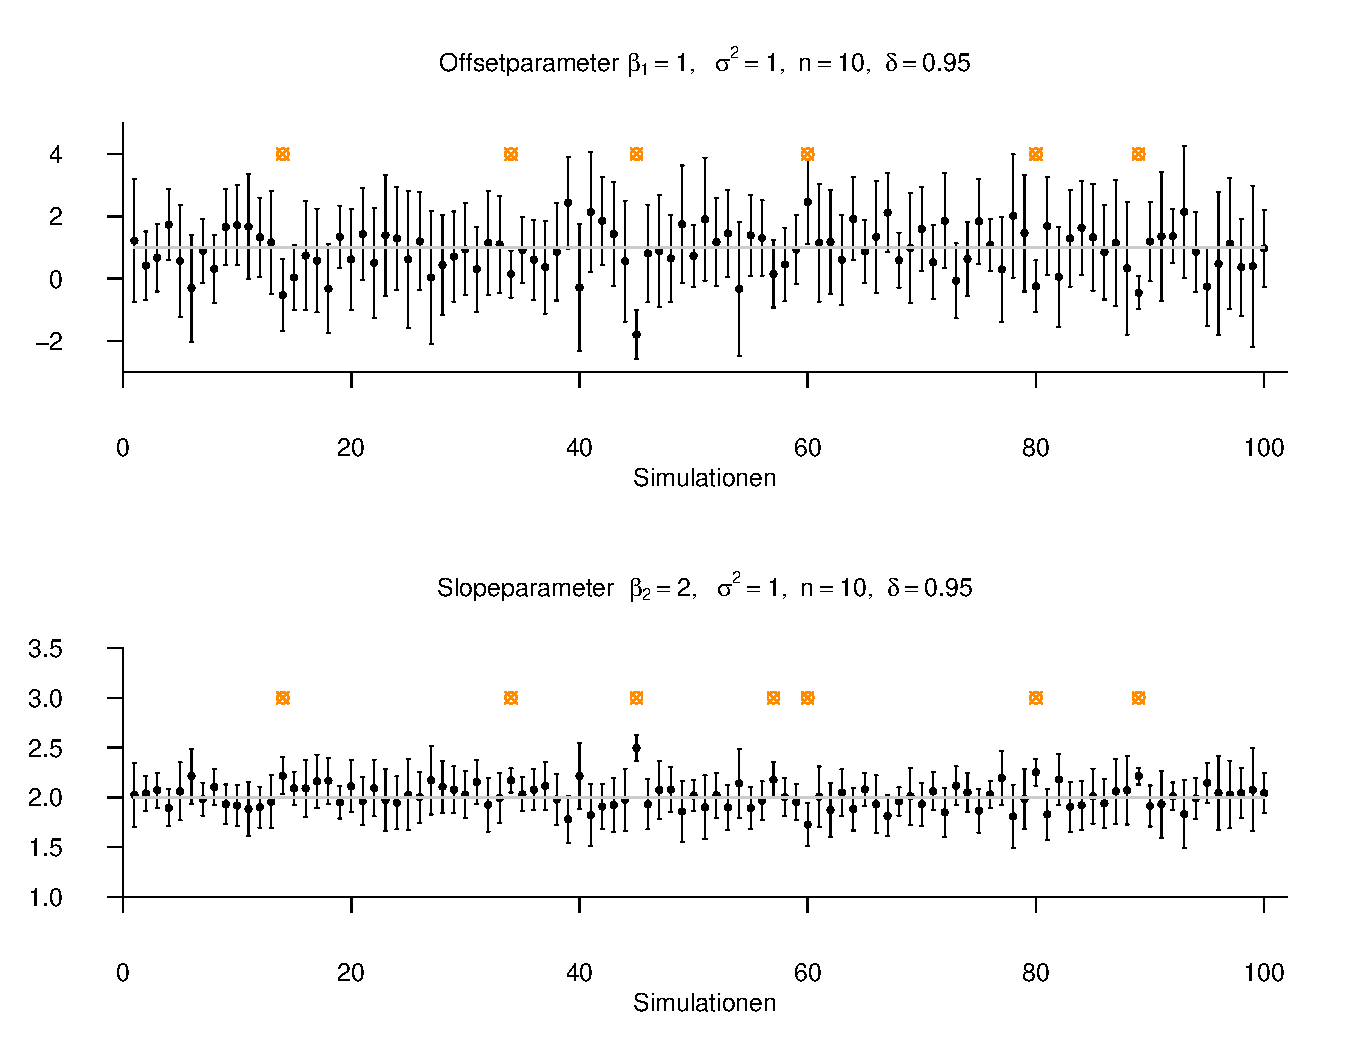
\includegraphics[width=0.9\linewidth]{7_Abbildungen/alm_7_elr_konfidenzintervalle} \end{center}
\end{frame}

\begin{frame}{}
\protect\hypertarget{section-12}{}
\vfill
\large
\setstretch{3}

T-Verteilungen

T-Statistiken

Konfidenzintervalle

\textbf{Selbstkontrollfragen} \vfill
\end{frame}

\begin{frame}{Selbstkontrollfragen}
\protect\hypertarget{selbstkontrollfragen}{}
\footnotesize
\setstretch{2.2}

\begin{enumerate}
\tightlist
\item
  Skizzieren Sie die WDFen von \(t\)-Zufallsvariablen mit 2, 10 und 30
  Freiheitsgraden.
\item
  Skizzieren Sie die WDFen von nichtzentralen \(t\)-Zufallsvariablen mit
  Nichtzentralitätsparametern 0,5 und 15.
\item
  Geben Sie die Definition der T-Statistik wieder.
\item
  Erläutern Sie für die T-Statistik die Bedeutung der Wahl von
  \(c \in \mathbb{R}^p\).
\item
  Erläutern Sie für die T-Statistik die Bedeutung der Wahl von
  \(\beta_0 \in \mathbb{R}^p\).
\item
  Wann und warum kann die T-Statistik als Signal-zu-Rauschen Verhältnis
  interpretiert werden?
\item
  Geben Sie das Theorem zur T-Statistik wieder.
\item
  Geben Sie die Form der T-Statistik im Szenario von \(n\) u.i.n.v.
  Zufallsvariablen wieder.
\item
  Erläutern Sie den Zusammenhang der T-Statistik und Cohen's \(d\).
\item
  Geben Sie das Theorem zu Konfidenintervallen für
  Betaparameterkomponenten wieder.
\end{enumerate}
\end{frame}

\begin{frame}{Referenzen}
\protect\hypertarget{referenzen}{}
\footnotesize
\setstretch{2.2}

\hypertarget{refs}{}
\begin{CSLReferences}{1}{0}
\leavevmode\vadjust pre{\hypertarget{ref-lehmann_1986}{}}%
Lehmann, E. L. 1986. \emph{Testing Statistical Hypotheses}. {Wiley
Series in Probability and Statistics}.

\leavevmode\vadjust pre{\hypertarget{ref-student_1908}{}}%
Student. 1908. {``The {Probable Error} of a {Mean}.''} \emph{Biometrika}
6 (1): 1--25.

\leavevmode\vadjust pre{\hypertarget{ref-zabell_2008}{}}%
Zabell, S. L. 2008. {``On {Student}'s 1908 {Article} {`{The Probable
Error} of a {Mean}'}.''} \emph{Journal of the American Statistical
Association} 103 (481): 1--7.
\url{https://doi.org/10.1198/016214508000000030}.

\end{CSLReferences}
\end{frame}

\end{document}
